
%----------------------------------------------------------------------------------------
% 	Template: Abschlussarbeiten des Studiengangs Angewandte Informatik an der HTW Berlin
% 	C. Schmidt 
%----------------------------------------------------------------------------------------
%	Pakete und Konfigurationen
%----------------------------------------------------------------------------------------
%\documentclass[twoside,twocolumn]{article}
%\documentclass[german,a4paper,12pt,oneside]{scrbook}
\documentclass[oneside,bibliography=totocnumbered,BCOR=5mm]{scrbook}% Voreinstellungen entfernt.

\usepackage[latin1]{inputenc}
\usepackage{amsmath, amsthm, amssymb}
\usepackage[ngerman]{babel}
%\usepackage[english]{babel} % Language hyphenation and typographical rules
\usepackage{marvosym}
\usepackage{graphics}
\usepackage{csquotes}
\newtheorem{satz}{Satz}[chapter]
\theoremstyle{definition} 
\newtheorem{definition}[satz]{Definition} 
\theoremstyle{definition} 
\newtheorem{lemma}[satz]{Lemma} 
\theoremstyle{definition} 
\newtheorem{bemerkung}[satz]{Bemerkung}
\theoremstyle{definition} 
\newtheorem{korollar}[satz]{Korollar} 
\theoremstyle{definition}
\newtheorem{beispiel}[satz]{Beispiel} 
\theoremstyle{definition} 
\newtheorem{algorithmus}{Algorithmus} 
\newenvironment{beweis}{\begin{proof}[Beweis]}{\end{proof}}
\usepackage[hyphens]{url}
\usepackage{hyperref}

%----------------------------------------------------------------------------------------
%	BIB.-Datei und Quellenverwaltung
%----------------------------------------------------------------------------------------
\usepackage[backend=bibtex, style=numeric]{biblatex}
\addbibresource{template.bib}
%\usepackage{natbib} % use natbib for references 
%----------------------------------------------------------------------------------------
\usepackage{blindtext} % Package to generate dummy text throughout this template 

\usepackage[sc]{mathpazo} % Use the Palatino font
\usepackage[T1]{fontenc} % Use 8-bit encoding that has 256 glyphs
\linespread{1.05} % Line spacing - Palatino needs more space between lines
\usepackage{microtype} % Slightly tweak font spacing for aesthetics

\usepackage[hmarginratio=1:1,top=32mm,columnsep=20pt]{geometry} % Document margins
\usepackage[hang, small,labelfont=bf,up,textfont=it,up]{caption} % Custom captions under/above floats in tables or figures
\usepackage{booktabs} % Horizontal rules in tables
\usepackage{lettrine} % The lettrine is the first enlarged letter at the beginning of the text
\usepackage{enumitem} % Customized lists
\setlist[itemize]{noitemsep} % Make itemize lists more compact

%\usepackage{abstract} % Allows abstract customization
%\renewcommand{\abstractnamefont}{\normalfont\bfseries} % Set the "Abstract" text to bold
%\renewcommand{\abstracttextfont}{\normalfont\small\itshape} % Set the abstract itself to small italic text

\usepackage{titlesec} % Allows customization of titles
%\renewcommand\thesection{\Roman{section}} % Roman numerals for the sections
%\renewcommand\thesubsection{\roman{subsection}} % roman numerals for subsections
%\titleformat{\section}[block]{\large\scshape\centering}{\thesection.}{1em}{} % Change the look of the section titles
%\titleformat{\subsection}[block]{\large}{\thesubsection.}{1em}{} % Change the look of the section titles

%\usepackage{fancyhdr} % Headers and footers
%\pagestyle{fancy} % All pages have headers and footers
%\fancyhead{} % Blank out the default header
%\fancyfoot{} % Blank out the default footer
%\fancyhead[C]{Ethics in Progress (EiP) $\bullet$ 2019 } % Custom header text
%\fancyfoot[RO,LE]{\thepage} % Custom footer text

\usepackage{titling} % Customizing the title section

%----------------------------------------------------------------------------------------
%	Listings
%----------------------------------------------------------------------------------------
\usepackage{listings}
\usepackage{color}

\definecolor{mygreen}{rgb}{0,0.6,0}
\definecolor{mygray}{rgb}{0.5,0.5,0.5}
\definecolor{mymauve}{rgb}{0.58,0,0.82}

\lstset{ 
  backgroundcolor=\color{white},   % choose the background color; you must add \usepackage{color} or \usepackage{xcolor}; should come as last argument
  basicstyle=\footnotesize,        % the size of the fonts that are used for the code
  breakatwhitespace=false,         % sets if automatic breaks should only happen at whitespace
  breaklines=true,                 % sets automatic line breaking
  captionpos=b,                    % sets the caption-position to bottom
  commentstyle=\color{mygreen},    % comment style
  deletekeywords={...},            % if you want to delete keywords from the given language
  escapeinside={\%*}{*)},          % if you want to add LaTeX within your code
  extendedchars=true,              % lets you use non-ASCII characters; for 8-bits encodings only, does not work with UTF-8
  firstnumber=1,                % start line enumeration with line 1000
  frame=single,	                   % adds a frame around the code
  keepspaces=true,                 % keeps spaces in text, useful for keeping indentation of code (possibly needs columns=flexible)
  keywordstyle=\color{blue},       % keyword style
  language=Octave,                 % the language of the code
  morekeywords={*,...},            % if you want to add more keywords to the set
  numbers=left,                    % where to put the line-numbers; possible values are (none, left, right)
  numbersep=5pt,                   % how far the line-numbers are from the code
  numberstyle=\tiny\color{mygray}, % the style that is used for the line-numbers
  rulecolor=\color{black},         % if not set, the frame-color may be changed on line-breaks within not-black text (e.g. comments (green here))
  showspaces=false,                % show spaces everywhere adding particular underscores; it overrides 'showstringspaces'
  showstringspaces=false,          % underline spaces within strings only
  showtabs=false,                  % show tabs within strings adding particular underscores
  stepnumber=1,                    % the step between two line-numbers. If it's 1, each line will be numbered
  stringstyle=\color{mymauve},     % string literal style
  tabsize=2,	                   % sets default tabsize to 2 spaces
  title=\lstname                   % show the filename of files included with \lstinputlisting; also try caption instead of title
}

%----------------------------------------------------------------------------------------
%	Haupttextteil
%----------------------------------------------------------------------------------------

\begin{document}

% Titelseite
% \pagestyle{empty}       % keine Seitennummer
\begin{titlepage}
\begin{center}

\includegraphics{HTW_Berlin_Logo_farbig.jpg}
\linebreak[4]
\linebreak[4]
\linebreak[4]
\linebreak[4]
\textit{\large Titel der Abschlussarbeit}
\linebreak[4]
\linebreak[4]
\linebreak[4]
Abschlussarbeit 
\linebreak[4]
\linebreak[4]
zur Erlangung des akademischen Grades: 
\linebreak[4]
\linebreak[4]
\textbf{Bachelor of Science (B.Sc.)} oder \textbf{Master of Science (M.Sc.)}
\linebreak[4]
\linebreak[4]
an der
\linebreak[4]
\linebreak[4]
Hochschule f\"ur Technik und Wirtschaft (HTW) Berlin
\linebreak[4]
Fachbereich 4: Informatik, Kommunikation und Wirtschaft
\linebreak[4]
Studiengang \textit{Angewandte Informatik}
\linebreak[4]
\linebreak[4]
\linebreak[4]
1. Gutachter\_in: Titel akademischer Grad Vorname Nachname\linebreak[4]
2. Gutachter\_in: Titel akademischer Grad Vorname Nachname\linebreak[4]
\linebreak[4]
\linebreak[4]
\linebreak[4]
\linebreak[4]
Eingereicht von Vorname Nachname [Matrikelnr.]
\linebreak[4]
\linebreak[4]
\linebreak[4]
\linebreak[4]
Datum

\end{center}
\end{titlepage}
\newpage    % Seitenwechsel

\thispagestyle{empty}       % keine Seitennummer
% vertikaler Leerraum
\vspace*{2.2cm}
\noindent %kein Einzug
{\Huge Danksagung}\\
\vspace*{1.6cm} \\

% Kopfzeilen (automatisch erzeugt)
%\pagestyle{headings}
[Text der Danksagung]

% Seite mit Abstracts
\newpage
\thispagestyle{empty}       % keine Seitennummer
\section*{Zusammenfassung}
[Text der Zusammenfassung]

\section*{Abstract}
[Summary of the thesis]


\clearpage
%Seite 1
\pagenumbering{roman}% Seitennummerierung "roemisch"
%\setcounter{page}{1} 

\tableofcontents  


%Seite 

 \listoffigures
 
 %Seite 6

 \listoftables
 


 \lstlistoflistings

.


\newpage

\pagenumbering{arabic}  % Nummerierung der Seiten in 'arabisch' % neues Kapitel mit Namen "Introduction"
 %Seite 1
 % \setcounter{page}{1}   % setzt Seitenzaehlung auf 1
 
 \chapter{Einleitung}
\fbox{\parbox{\linewidth}{
Vorliegendes Template enth\"alt exemplarisch (und damit unvollst\"andig) Gliederungspunkte, Bestandteile und Hinweise f\"ur ein typisches Softwareentwicklungsprojekt, bei dem ein Prototyp erstellt wird. Es dient als Hilfestellung zu Ihrer weiteren Verwendung. Selbstverst\"andlich m\"ussen Sie selbst weitere Erg\"anzungen und Anpassungen vornehmen.

\begin{center}
\textbf{Viel Erfolg sowie gutes Gelingen bei Ihrer Abschlussarbeit!}
\end{center}
}}
\\
\linebreak[4]
\linebreak[4]
Der Textteil beginnt hier und wird arabisch mit dieser Seite beginnend mit \frqq1\flqq{} arabisch nummeriert. Der Textteil gliedert sich in Kapitel und Unterkapitel. Soll jede Hierarchieebene benannt werden, dann ist folgende Terminologie  \"ublich:

\begin{itemize}
\item 1. Hierarchieebene: Hauptkapitel
\item 2. Hierarchieebene: Kapitel
\item 3. Hierarchieebene: Unterkapitel
\item 4. Hierarchieebene: Abschnitt
\end{itemize}

Der inhaltliche Aufbau einer Abschlussarbeit im Studiengang \textit{Angewandte Informatik} h\"angt selbstverst\"andlich vom Thema und vom Inhalt ab. Abweichungen von der diesem Template zu Grunde liegenden Gliederungsstruktur sind immer m\"oglich, manchmal sogar zwingend notwendig. Stimmen Sie sich diesbez\"uglich immer mit Ihren Gutachter(inne)n ab.


Vergessen Sie niemals, all Ihre verwendeten Quellen anzugeben und korrekt zu zitieren\footnote{Erg\"anzende Informationen k\"onnen Sie auch in eine Fu"snote auslagern. Hier wird die Fu"snote dazu genutzt, um Ihnen bei Interesse am Thema Zitation vertiefende Quellen (z.B. \autocite{balzert2011} oder \autocite{franck2013}) anzubieten.}. Quellen k\"onnen manuell referenziert und im Quellenverzeichnis eingetragen werden. Erg\"anzend bieten viele Textverarbeitungsssteme auch ausgelagerte Quellenverwaltungsdateien und - systeme an,  \"uber die mittels entsprechender Befehle im Textteil zitiert werden kann\footnote{Wie Sie hoffentlich feststellen werden, erfolgt die Literaturverwaltung in diesem Template mittels einer *.bib-Datei (diese enth\"alt die verwendeten Quellen), welche die *.tex-Datei mittels Verwendung von biblatex und bibtex erg\"anzt.}.

Visualisieren Sie im Textteil angemessen, z.B. mittels Abbildungen und Tabellen. Vorliegendes Template enth"alt beispielhaft eingebundene Abbildungen und eine Tabelle (vgl. f.), welche der Steinlausforschung\footnote{Analog zu Straube (In: \autocite{pschy}) handelt es sich bei der Steinlaus (\textit{petrophaga lorioti}) um das \frqq \textit{kleinste einheimische Nagetier}\flqq. Als stimmungsaufhellender Endoparasit erreicht es eine Gr\"o"se von ca. 0,3 bis 3 mm und stammt aus der Familie der Lapivora. Die Steinlaus kommt ubiquit\"ar vor und ist in der Regel apathogen.} entnommen sind.


\begin{figure}
\centering
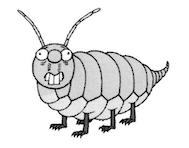
\includegraphics{steinlaus.jpg}
  \caption{Beispielgrafik: Steinlaus; Bildquelle \autocite{loriot}}
\end{figure}



\begin{figure}
\centering
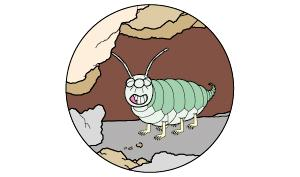
\includegraphics{steinlaus2.jpg}
  \caption{Beispielgrafik: Fressende Steinlaus; Bildquelle \autocite{loriot2}}
\end{figure}

\begin{table}
\caption{\"Ubersicht: Untersuchte Steinl\"ause}
\centering
\begin{tabular}{llr}
\toprule
\multicolumn{2}{c}{Untersuchte Objekte mit Lokation des Habitats} \\
\cmidrule(r){1-2}
ID (nickname) & Ort & Gr\"o"se/L\"ange (in mm) \\
\midrule
1 (Rosalinde) & Berlin, Mauerpark & $1.4$ \\
2 (Devil in disguise) & Brandenburg, BER-Airport & $2.8$ \\
3 (Hannes) & Berlin, Olympia-Stadion & $2.1$ \\
4 (Her Majesty) & Berlin, Humboldt-Forum & $2.0$ \\
\bottomrule
\end{tabular}
\end{table}

\section{Hintergrund der Arbeit}
[Beschreibung des groben Kontextes der Arbeit; im Detail sollten Sie dies im Grundlagenteil darstellen] 


\section{Problem- und Zielstellung (Scope)}
[Beschreibung der Problemstellung sowie der sich daraus ergebenden Teilprobleme,-ziele und Forschungsfrage(n), welche Sie mit Ihrer Arbeit addressieren]


\section{Aufbau der Arbeit}
[Beschreibung des Aufbaus der Arbeit]


\chapter{Grundlagen}
[Beschreibung des Kontextes der Arbeit mit allen durch die Problemstellung tangierten Bereichen, Methoden, Theorien, Erkenntnissen, Technologien, ... ] 


\section{Kontext}


\subsection{Domain} 



\subsection{Technologien}


\subsection{Methoden und Konzepte}


\section{...}


\subsection{...}


\subsection{...}

\chapter{Methodologie}

[Beschreibung des geplanten Vorgehens(-modells) zur L\"osung der Problemstellung; umfasst u.a.:
\begin{itemize}
\item Anforderungserhebung und -analyse
\item Konzeption, Entwurf
\item Umsetzung (Implementierung)]
\end{itemize}

\section{Ergebnisartefakte}
[Beschreibung der Ergebnisse / Ergebnistypen, welche Sie im Rahmen der Probleml\"osung generieren / erzielen wollen, z.B. Algorithmus, Prototyp einer Software(komponente), ... ]

\section{Datenschutzaspekte}
[Beschreibung von Aspekten des Datenschutzes im Zusammenhang mit Ihrer Abschlussarbeit]

\section{Ethische Aspekte}
[Beschreibung von Aspekten der Ethik\footnote{vgl. hierzu erg\"anzend allgemeine Codizes (z.B. \autocite{acm}, \autocite{ieee} oder \autocite{gi}) sowie auch domain-spezifische Normen und Verfahrensweisen im Rahmen einer kritischen Reflektion.}im Zusammenhang mit Ihrer Abschlussarbeit]



\chapter{Anforderungserhebung und -analyse}
[Beschreibung der Erhebung, Granularisierung und Priorisierung der zu Grunde liegenden Anforderungen]
\section{Nutzer- und Systemanforderungen}
\subsection{Funktionale Anforderungen}
\subsubsection{Obligatorisch (MUSS)}
\subsubsection{Fakultativ (Kann)}
\subsection{Nicht-funktionale Anforderungen}

\subsubsection{Obligatorisch (MUSS)}
\subsubsection{Fakultativ (Kann)}
\section{...}




\chapter{Konzeption \& Entwurf}
[Beschreibung des Entwurfs auf Basis der Methodologie / der geplanten Vorgehensweise zur Probleml\"osung im Kontext der Anforderungen (i.A. der Art der Arbeit)]
\section{Prozess}
\section{Systemarchitektur}
\section{Softwarearchitektur}
\section{Schnittstellen}
\section{Datenmanagement}
\section{...}



\chapter{Implementierung}

[Beschreibung der Implementierung\footnotemark auf Basis des Entwurfs und der Methodologie / der geplanten Vorgehensweise zur Probleml\"osung im Kontext der Anforderungen. Hier ist Raum f\"ur Listings, wie z.B. das nun Folgende:


\footnotetext{Beachten Sie bei der Implementierung und deren Dokumentation bitte Clean Code Empfehlungen (vgl. hierzu z.B. \autocite{martin2008}).} 

\begin{lstlisting}[caption={Ein Beispiel: Hello World (Scala)}]
object HelloWorld {
  def main(args: Array[String]): Unit = {
    println("Hello, world!")
  }
}
\end{lstlisting}

Umfangreicher Quell-Code sollte in den Anhang ausgelagert werden.]


\chapter{Test}
[Beschreibung, wie Sie auf Basis des geplanten Testvorgehens was mit welchen Kriterien und Technologien getestet haben]

\chapter{Darstellung und Bewertung der Ergebnisse}
[Beschreibung der Ergebnisse aus allen voran gegangenen Kapiteln sowie der zuvor generierten Ergebnisartefakte mit Bewertung, wie diese einzuordnen sind]

\chapter{Zusammenfassung}
[Aggregierte retrograde Kurzbeschreibung der Arbeit]
\section{Schlussfolgerungen}
[Beschreibung der insgesamt zu konstatierenden Schlussfolgerungen im Zusammenhang mit der Arbeit]
\section{Limitationen}
[Beschreibung der Ergebnisse einer kritischen Reflektion und Begr\"undung dessen, was die Arbeit nicht zu leisten vermag]
\section{Ausblick}
[Beschreibung und Begr\"undung potenzieller zuk\"unftiger Folgeaktivit\"aten im Zusammenhang mit Ihrer Arbeit (z.B. weitere Anforderungen, Theoriebildung, ... ]
























%----------------------------------------------------------------------------------------
%	REFERENCE LIST
%----------------------------------------------------------------------------------------


% \bibliographystyle{apalike}
% \bibliographystyle{ksfh_nat} % ein anderer Stil
% \bibliography{science} 

%\begin{thebibliography}{XX}
%\bibitem[Bielecki, Rutkowski(2002)]{bielecki02}T. Bielecki, M. Rutkowski, Credit Risk: Modeling, Valuation and Hedging, Springer (2002).
%\bibitem[Jarrow, Turnbull(1995)]{jarrow95} R.A. Jarrow, S. Turnbull, Pricing derivatives on financial securities subject to credit risk, Journal of Finance, 50:1 (1995) 53--85.
%\bibitem[Marshall, Olkin(1967)]{marshall67} A.W. Marshall, I. Olkin, A multivariate exponential distribution, Journal of the American Statistical Association, 62 (1967), pp. 30--44.
%\bibitem[Sch\"onbucher(2003)]{schoenbucher03} P.J. Sch\"onbucher, Credit Derivatives Pricing Models, Wiley (2003).
%\end{thebibliography}

\printbibliography[
heading=bibintoc,
title={Quellenverzeichnis}
]


\newpage

\chapter{Abk\"urzungsverzeichnis}
\newpage
\chapter{Glossar}




\begin{appendix}

\pagenumbering{Roman}

\chapter{Appendix}


\section{Quell-Code}

\section{Tipps zum Schreiben Ihrer Abschlussarbeit}

\begin{itemize}
\item Achten Sie auf eine neutrale, fachliche Sprache. Keine \glqq{}Ich\grqq{}-Form.
\item Zitieren Sie zitierf\"ahige und -w\"urdige Quellen (z.B. wissenschaftliche Artikel und Fachb\"ucher; nach M\"oglichkeit keine Blogs und keinesfalls Wikipedia\footnote{Wikipedia selbst empfiehlt, von der Zitation von Wikipedia-Inhalten im akademischen Umfeld Abstand zu nehmen \autocite{wikipedia2019}.}). 
\item Zitieren Sie korrekt und homogen.
\item Verwenden Sie keine Fu{\ss}noten f\"ur die Literaturangaben.
\item Recherchieren Sie ausf\"uhrlich den Stand der Wissenschaft und Technik.
\item Achten Sie auf die Qualit\"at der Ausarbeitung (z.B. auf Rechtschreibung).
\item Informieren Sie sich ggf. vorab dar\"uber, wie man wissenschaftlich arbeitet bzw. schreibt:
\begin{itemize}
\item Mittels Fachliteratur\footnote{Z.B. \autocite{balzert2011}, \autocite{franck2013}}, oder
\item Beim Lernzentrum\footnote{Weitere Informationen zum Schreibcoaching finden sich hier: \url{https://www.htw-berlin.de/studium/lernzentrum/studierende/schreibcoaching/}; letzter Zugriff: 13 VI 19.}.
\end{itemize}
\item Nutzen Sie \LaTeX\footnote{Kein Support bei Installation, Nutzung und Anpassung allf\"alliger \LaTeX-Templates!}.
\end{itemize}



\newpage
% Letzte Seite
\thispagestyle{empty}       % keine Seitennummer
%\vspace*{18cm}
\noindent

\section*{Eidesstattliche Versicherung}
Hiermit versichere ich an Eides statt durch meine Unterschrift, dass ich die vorstehende Arbeit selbstst\"andig und ohne fremde Hilfe angefertigt und alle Stellen, die ich w\"ortlich oder ann\"ahernd w\"ortlich aus Ver\"offentlichungen entnommen habe, als solche kenntlich gemacht habe, mich auch keiner anderen als der angegebenen Literatur oder sonstiger Hilfsmittel bedient habe. Die Arbeit hat in dieser oder \"ahnlicher Form noch keiner anderen Pr\"ufungsbeh\"orde vorgelegen.\\
\linebreak[4]
\linebreak[4]
\linebreak[4]
\linebreak[4]
-------------------------------------------------------\linebreak[4]
Datum, Ort, Unterschrift


\end{appendix}


\end{document}

